\section{Implementation of Tessevolve}

Here we describe in depth the data model, design choices, and implementation features involved in the development of Tessevolve. Our visualization makes use of 3D projections in virtual reality to scale up the fitness landscape metaphor into multiple dimensions. We use the emerging digital evolution platform MABE2 to generate evolutionary data, the ALife Data Standards Python package to process lineage information, and the open-source platforms A-Frame, D3.js, and Bootstrap to create easily accessible web and VR interfaces for the final data visualization. The result is a fully open source visualization of complex, multidimensional phylogenetic and evolutionary data. The full GitHub repository for the project, including all scripts involved in data generation, pre-processing, and visualization, is available at \url{https://github.com/alackles/tessevolve} \citep{ackles_alacklestessevolve_2022}, and the platform itself is accessible at \url{https://alackles.github.io/tessevolve}. Note that for all figures in this paper, due to the nature of the images, they would likely better be viewed at the live demo linked above.
% change github URL to DOI before submission

\subsection{Data Model}

Currently, there is no broadly accepted standard for fitness landscape data. Our data model therefore accepts data in CSV format, with initial columns \texttt{x0, x1, x2, x3} representing the traits of interest, and a column \texttt{fitness} which represents the fitness associated with those trait values. Columns \texttt{x2} and \texttt{x3} are optional dependent on the dimensionality of the underlying landscape (i.e., a 3D landscape would only have columns \texttt{x0, x1, x2, fitness}). 

We were also interested in visualizing lineages' evolution (phylogenetic data) across these fitness landscapes. Since in this case the data we visualized was from computationally evolved organisms, we use the ALife Data Standard for phylogenetic data \citep{lalejini_data_2019}. In this standard, information about an organisms's traits is recorded every time a new lineage forms. In the future, Tessevolve could be expanded to accept phylogenetic data in other formats such as the biologically-standard Newick format.

\subsection{Data Generation and Pre-Processing}

To generate the fitness landscapes used for our web demo of Tessevolve, we turned to the CEC'2013 Benchmark functions which provide both Python and C++ (among other languages) implementations of multiple functions across dimensions \citep{li_benchmark_2013}. The fitness landscape data itself was generated using the Python implementations, while the C++ implementations were incorporated into the digital evolution platform MABE2 (https://github.com/mercere99/MABE2) to generate lineage data. We then used the ALife Standards Python package to process the lineage data into a standardized CSV format for the visual front-end \citep{lalejini_data_2019}.

% I have no idea if we need to add more information here. 

\subsection{Virtual Reality Engine}

Virtual reality allows for users to take maximal ability of the brain's ability to build intuition about physical spaces. By being immersed in the visualization, they can develop a visceral understanding of how it behaves. However, to promote accessibility, it is ideal for VR visualizations to also be viewable in a web browser, as a fallback. By allowing web users to manipulate the visualization with their mouse, such a format can still provide a far better experience than a static 2D projection.

To this end, we chose to implement Tessevolve using the webXR specification, which supports browser-based VR scenes that can be viewed in a browser in addition to on a VR headset. Specifically, we used Mozilla's AFrame framework \citep{mozilla_-frame_2022}, which facilitates building a VR visualization out of html components. This structure allows it to play nicely with d3.js \citep{bostock_d_2011}, which we used to connect the data into the visualization.

\subsection{Design Choices}

The most crucial design decision we had to make was how to display the 3D landscape in a way that was both intuitive and informative. In particular, we needed to decide how users would be able to see multiple points in a landscape simultaneously. For example, a true 3D analogue to the traditional 2D landscape would be akin to an aquarium tank, where every spot in the 3D space conveys some visual information about the fitness at that point. However, such a design would completely block the vision of the viewer when they are inside the landscape; there is no space to see ``around" any component to investigate other regions (\autoref{fig:imp:spheres}) 

\begin{figure}
    \centering
    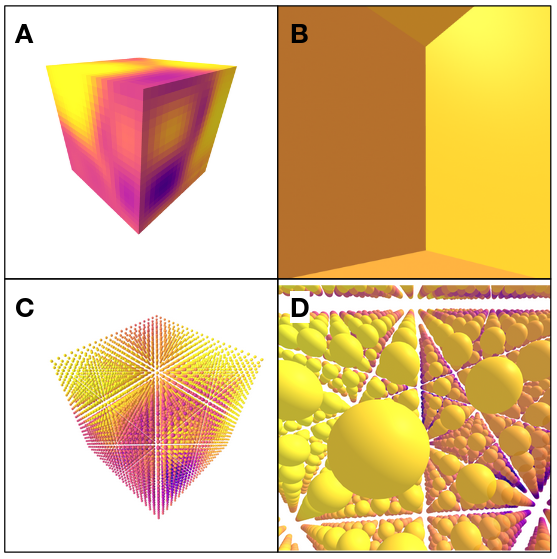
\includegraphics[width=0.5\textwidth]{chapters/3-vr-viz/figs/spheres.png}
    \caption{Illustration of the challenges of having a continuous 3D landscape visualization. (A) A landscape visualization where all genotypes are displayed. (B) The poor view from inside \textit{A}. (C) A landscape visualization where genotypes are displayed at fixed, discrete intervals. (D) The view from inside \textit{C}.}
    \label{fig:imp:spheres}
\end{figure}

We therefore chose to display discrete, evenly-spaced points on the landscape rather than a continuous mesh. These points are displayed as spheres at 90\% opacity, allowing for both distant and nearby inspection of the landscape. While this technique somewhat reduces the resolution of the fitness landscape, it greatly increases its interpretability. 

Another challenge was how to indicate the fitness at each point when all three of our spatial dimensions are used to convey information about trait values. For this purpose, we use a color scale, as is commonly implemented to visualize imaginary functions. This method should be easily recognizable to domain experts due to its frequent use in other mathematical visualizations. We chose to use the viridis color scheme plasma variant as it is both colorblind friendly and maps ``cool" colors to low values and ``warm" colors to high values, further increasing familiarity.

We also wanted to display lineage data on landscapes. We represent newly born taxa as cubes to distinguish from the landscape's spheres, and consecutive taxa are connected by a simple line. The color scheme for the fitness of each taxon is the same as that of the landscape. 

\subsection{Visualization Interface}


\begin{figure*}
    \centering
    \fbox{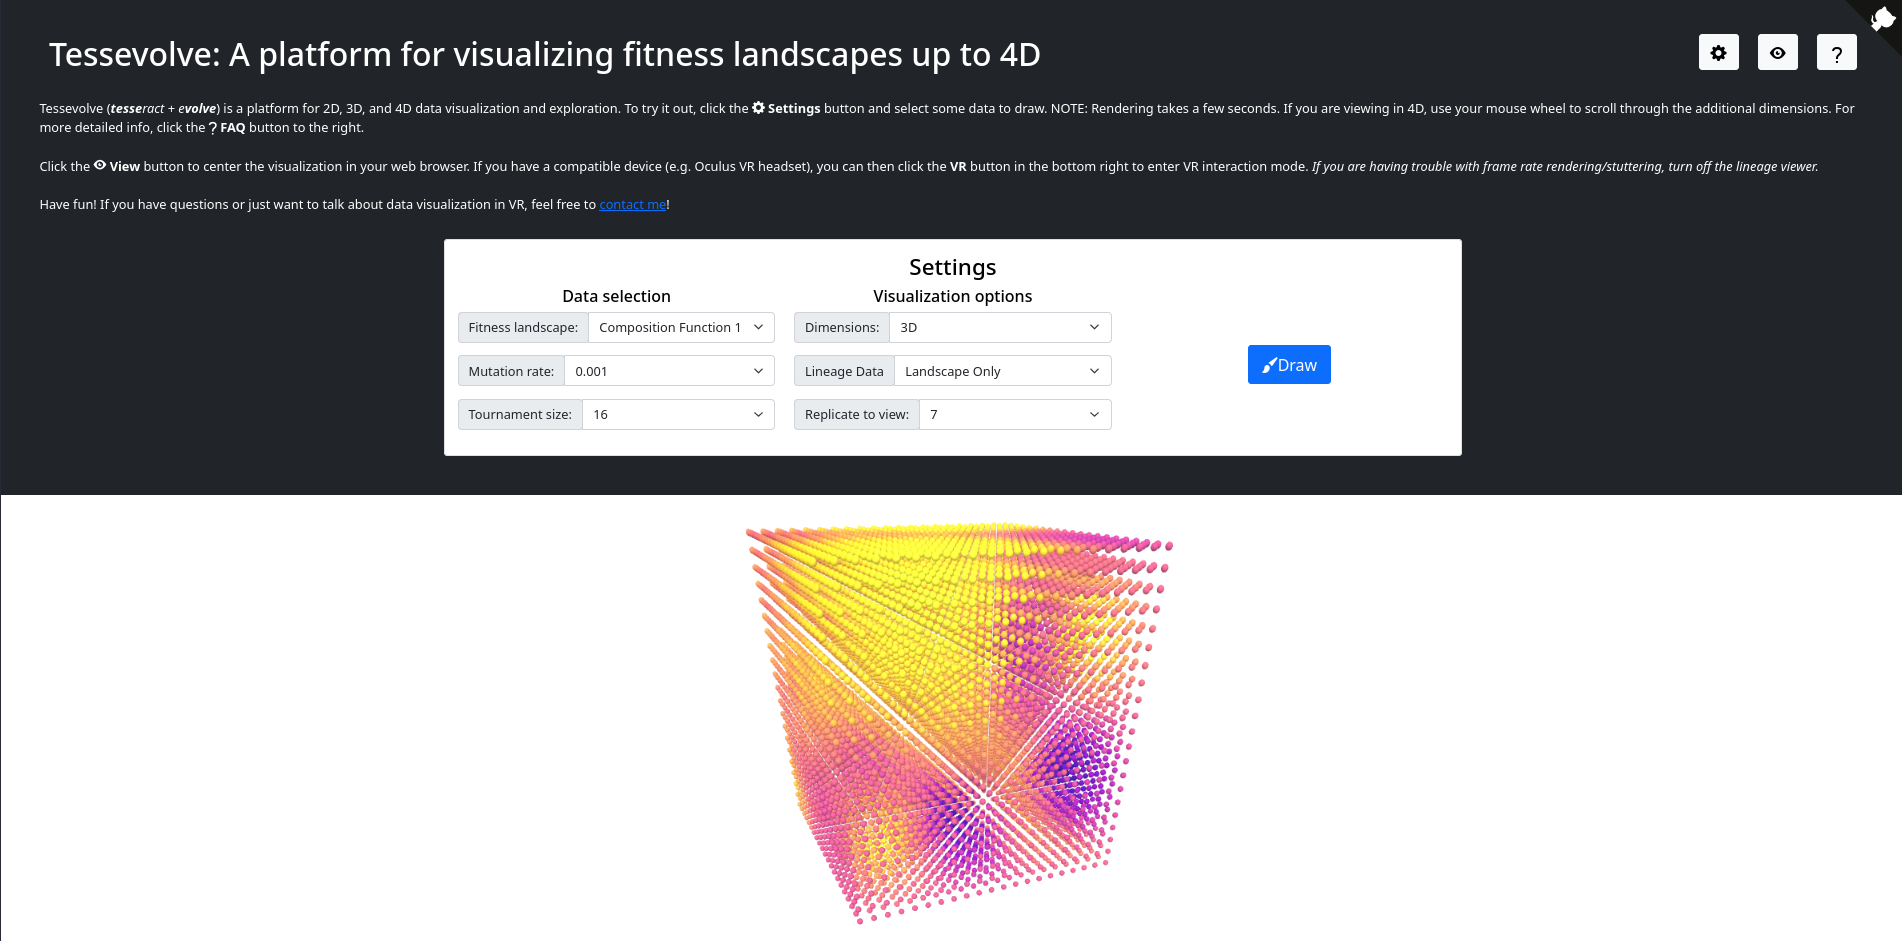
\includegraphics[width=\textwidth]{chapters/3-vr-viz/figs/tessevolve.png}}
    \caption{Tessevolve web interface. Changing the settings in the settings drop-down panel and clicking `Draw' allows users to load an updated landscape. The FAQ provided in the top right contains detailed information about the display. Drop-down menus allow users to select the combinations of parameters they are interested in seeing; the Draw button loads that configuration into the JavaScript DOM. The configuration of settings shown here is used in all other figures unless otherwise stated.}
    \label{fig:imp:tessevolve}
\end{figure*}


Tessevolve is available through any modern web browser at \url{https://alackles.github.io/tessevolve}.

The front-end interface for Tessevolve is a simple interactive web page (\autoref{fig:imp:tessevolve}). The top banner contains brief information about the site, displays for additional info, and a settings panel. Under the settings panel is an embedded A-Frame scene which can be adjusted to fill the screen or, in a VR headset, sent to VR mode. 

Under the hood, the site stores pre-processed landscape and lineage data for several evolutionary conditions and replicates. When users adjust the settings in the settings panel and click the Draw button to cue the site to reload, the embedded scene clears the old data and loads the new. 

The result is a 3D projection of the selected landscape. Users on the web version can navigate around the projection with the WASD or arrow keys and change viewing direction using the mouse; in VR, they can move with the left joystick or by walking around the space. 

\subsection{Dimension Comparisons}

Users can view the same landscape and its associated lineage in 2D, 3D, or 4D. Each dimension has its own unique design choices to help build intuition about extension into higher dimensions.

\subsubsection{2D Landscapes}

2D landscapes are displayed as a vertical grid of spheres in 3D space. Trait values are mapped to vertical and horizontal coordinates, while fitness is mapped to the Plasma color scheme (FIG). These landscapes are simple enough that they could be represented using the traditional relief map technique,  where fitness is used as a third dimension; see for example \autoref{fig:related-work:2dviz}. However, to keep visualization consistent across dimensions and maintain the analogy from 2D to 3D and 3D to 4D, 2D landscapes here are instead shown as if they were a single ``slice" of a 3D landscape. 

Lineage data is displayed as cubes connected by lines. Each cube represents the birth of a new \textit{taxon}---that is, in this case, a novel trait value. Cube positions represent trait values and color represents fitness; lines connect consecutive taxa. 

\subsubsection{3D Landscapes}

3D landscapes are displayed as an evenly-spaced mesh of spheres in 3D space. As in 2D, traits and fitness are mapped to position and color respectively in both landscapes and lineages. The only difference between the 2D and 3D landscape visualizations is the additional dimension.

\subsubsection{4D Landscapes}

4D landscapes required more complex design choices to account for the fourth dimension, which cannot be displayed concurrent with the other three. Here, the user sees one 3D ``slice" of the landscape at a time, and can move through the slices by scrolling. Each slice represents a different value for the fourth dimension, and fitness is computed based on the total trait values across all four dimensions. The result is that the spheres' positions remain fixed, while the colors change across the landscape to represent how fitness is changing over each slice. This representation was loosely inspired by Bosch's 4D toy-box application \citep{bosch_n_2020}.

Lineage data also adjusts depending on the current 3D slice. The connections between nodes are always displayed, but the colors of the nodes are only displayed when that node falls on the currently-viewed slice. Otherwise, nodes are greyed out and transparent to indicate that they are not present in this slice.